% !TeX program = xelatex
% !TeX root = representation_final.tex
% !TeX encoding = UTF-8
% !TeX spellcheck = en_US
% arara: xelatex: { interaction: nonstopmode, synctex: yes }
% arara: xelatex: { interaction: nonstopmode, synctex: yes }
%
% Auto-build note:
% - VS Code LaTeX Workshop: enable "latex-workshop.latex.autoBuild.run": "onSave".
% - TeXstudio/TeXShop can use the magic comments above to choose XeLaTeX.
% - Manual command from final_submission/:
%   bash watch_representation_final.sh
% - Automatic watch (save-to-recompile):
%   bash watch_representation_final.sh representation_final.tex

\documentclass[aspectratio=169,10pt]{beamer}

\usepackage{fontspec}
\usepackage{graphicx}
\usepackage{booktabs}
\usepackage{array}
\usepackage{tabularx}
\usepackage{amsmath,amssymb}
\usepackage{xcolor}
\usepackage{tikz}
\usetikzlibrary{arrows.meta,positioning,calc}

\graphicspath{{figures/}}

% Fudan-inspired, projector-safe palette.
\definecolor{fudanblue}{HTML}{0B4EA2}
\definecolor{fudanmid}{HTML}{2F68B2}
\definecolor{fudanlight}{HTML}{EEF4FC}
\definecolor{textgray}{HTML}{333333}
\definecolor{mutedgray}{HTML}{6B7280}
\definecolor{rulegray}{HTML}{D7DCE5}
\definecolor{accentorange}{HTML}{D97904}
\definecolor{accentgreen}{HTML}{008A5B}

\newcommand{\pos}[1]{\textcolor{fudanblue}{#1}}
\newcommand{\warn}[1]{\textcolor{accentorange}{#1}}
\newcommand{\HL}[1]{\textcolor{accentgreen}{#1}}

\setbeamertemplate{navigation symbols}{}
\setbeamersize{text margin left=0.72cm,text margin right=0.72cm}
\setbeamercolor{normal text}{fg=textgray,bg=white}
\setbeamercolor{frametitle}{fg=fudanblue,bg=white}
\setbeamercolor{item}{fg=fudanblue}
\setbeamercolor{caption name}{fg=fudanblue}
\setbeamerfont{frametitle}{series=\bfseries,size=\Large}
\setbeamerfont{framesubtitle}{size=\small}
\setbeamerfont{title}{series=\bfseries,size=\LARGE}
\setbeamerfont{subtitle}{size=\large}
\setbeamerfont{itemize/enumerate body}{size=\small}
\setbeamerfont{itemize/enumerate subbody}{size=\small}

\setbeamertemplate{itemize item}{\color{fudanblue}\scriptsize$\blacksquare$}
\setbeamertemplate{itemize subitem}{\color{fudanblue}\scriptsize$\blacktriangleright$}

\newcommand{\maybelogo}[2]{%
  \IfFileExists{figures/#1}{\includegraphics[#2]{#1}}{}%
}

\newcommand{\fig}[2][]{%
  \IfFileExists{figures/#2}{\includegraphics[#1]{#2}}{%
    \fbox{\begin{minipage}[c][0.34\textheight][c]{0.94\linewidth}
      \centering\small Missing figure:\\ \texttt{\detokenize{figures/#2}}
    \end{minipage}}%
  }%
}

\newcommand{\keyline}[1]{%
  \vspace{0.04cm}
  \noindent\begin{tabular}{@{}m{2.2pt}@{\hspace{0.55em}}m{0.90\linewidth}@{}}
    {\color{accentgreen}\rule{2.2pt}{1.35em}} & \textbf{#1}
  \end{tabular}
  \vspace{0.09cm}
}

\newcommand{\metric}[2]{%
  \begin{minipage}[t]{0.30\linewidth}
    \centering
    {\Large\bfseries\color{fudanblue}#1}\\[-1pt]
    {\scriptsize\color{mutedgray}#2}
  \end{minipage}
}

\newcommand{\smallnote}[1]{%
  {\scriptsize\color{mutedgray}#1}
}

\setbeamertemplate{frametitle}{%
  \begin{tikzpicture}[remember picture,overlay]
    \node[anchor=north west,inner sep=0pt] at ($(current page.north west)+(0.78cm,0cm)$)
      {\maybelogo{fudan_logo.png}{height=1.34cm}};
    \node[anchor=north west,align=left,text width=0.74\paperwidth] at ($(current page.north west)+(2.58cm,-0.47cm)$)
      {{\usebeamerfont{frametitle}\color{fudanblue}\insertframetitle\par}
       {\usebeamerfont{framesubtitle}\color{fudanblue!72!black}\insertframesubtitle\par}};
  \end{tikzpicture}
  \vspace{1.42cm}
}

\setbeamertemplate{footline}{%
  \leavevmode
  \hbox{\hspace{0.72cm}\scriptsize\color{mutedgray}\insertframenumber/\inserttotalframenumber}
  \vspace{0.20cm}
}

\title{CNN Representation-Assisted MMMD}
\subtitle{From Power Improvement to Biomedical Domain-Shift Interpretation}
\author{Dechao's Individual Component}
\date{June 2026}


\begin{document}

{% title page
\begin{frame}[plain]
  \begin{tikzpicture}[remember picture,overlay]
    \fill[white] (current page.south west) rectangle (current page.north east);
    \begin{scope}
      \clip ($(current page.south east)+(-5.85cm,0cm)$) --
            ($(current page.north east)+(-2.62cm,0cm)$) --
            (current page.north east) --
            (current page.south east) -- cycle;
      \IfFileExists{figures/fudan_background.png}{%
        \node[anchor=south east,inner sep=0pt] at (current page.south east)
          {
\includegraphics[width=0.68\paperwidth,height=\paperheight]{fudan_background.png}};
      }{%
        \fill[fudanblue] (current page.south west) rectangle (current page.north east);
      }
    \end{scope}
    \node[anchor=north west,inner sep=0pt] at ($(current page.north west)+(0.78cm,0cm)$)
      {\maybelogo{fudan_logo.png}{height=1.75cm}};
    \node[anchor=north west,inner sep=0pt] at ($(current page.north west)+(0.88cm,-2.58cm)$) {%
      \begin{minipage}{0.60\paperwidth}
        \raggedright
        {\color{textgray}\usebeamerfont{title}\inserttitle\par}
        \vspace{0.20cm}
        {\color{textgray}\usebeamerfont{subtitle}\insertsubtitle\par}
        \vspace{0.58cm}
        {\color{textgray}\large\insertauthor\par}
        \vspace{0.12cm}
        {\color{textgray}\insertdate\par}
      \end{minipage}
    };
  \end{tikzpicture}
\end{frame}
}

% -------------------------------------------------------------------
\begin{frame}{MNIST Reproduction}{Original-paper benchmark check}
\begin{center}
\hspace*{0.3cm}\begin{minipage}{1.1\linewidth}
\begin{columns}[T,totalwidth=\linewidth]
\begin{column}{0.49\linewidth}
  \centering
  {\large\bfseries Power}\\[0.25em]
  \fig[width=\linewidth]{mnist_cnn_power.png}
\end{column}
\begin{column}{0.49\linewidth}
  \centering
  {\large\bfseries Type-I error}\\[0.25em]
  \fig[width=\linewidth]{mnist_cnn_type1_error_two_nulls.png}
\end{column}
\end{columns}
\end{minipage}
\end{center}
\vspace{-0.05cm}
\begin{center}
\smallnote{Reproduction anchor: MNIST additive-noise power plus matched-null calibration.}
\end{center}
\end{frame}

% -------------------------------------------------------------------
\begin{frame}{Representation Choice}{Raw pixels versus CNN embeddings for image two-sample testing}
\begin{columns}[T,totalwidth=\linewidth]

\begin{column}{0.60\linewidth}
  \vspace{-0.15cm}
  \fig[width=1.2\linewidth]{mnist_cnn_power.png}
\end{column}

\begin{column}{0.3\linewidth}

  \vspace{0.9em}
  \begin{itemize}
    \item Original MMMD improves kernel and bandwidth choice for a fixed input space.
    \item I compare raw pixels with CNN embeddings.
    \item Train CNN once, freeze it, cache embeddings, and run MMMD repeatedly.
    \item Multilayer variants: 3 components with one Gaussian per layer, or 15 components with five bandwidths per layer.
  \end{itemize}

\end{column}

\end{columns}
\end{frame}

% -------------------------------------------------------------------
\begin{frame}{CNN-MMMD}{A lightweight representation-assisted pipeline}
\keyline{Use MMMD on learned image features, not only on flattened pixels.}
\vspace{0.12cm}
\begin{center}
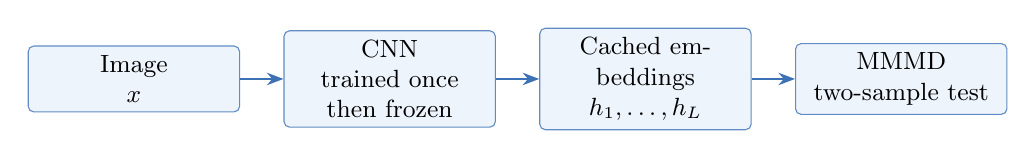
\begin{tikzpicture}[
  node distance=0.55cm,
  flowbox/.style={draw=fudanblue!65, fill=fudanlight, rounded corners=2pt,
                  minimum height=0.82cm, text width=2.45cm, align=center, font=\small},
  arr/.style={-{Stealth[length=2.1mm]}, thick, draw=fudanblue!80},
  note/.style={font=\scriptsize, color=mutedgray, align=center}
]
  \node[flowbox] (x) {Image\\$x$};
  \node[flowbox, right=of x] (cnn) {CNN trained once\\then frozen};
  \node[flowbox, right=of cnn] (emb) {Cached embeddings\\$h_1,\ldots,h_L$};
  \node[flowbox, right=of emb] (mmmd) {MMMD\\two-sample test};
  \draw[arr] (x) -- (cnn);
  \draw[arr] (cnn) -- (emb);
  \draw[arr] (emb) -- (mmmd);
\end{tikzpicture}
\end{center}
\vspace{0.08cm}
\begin{columns}[T,totalwidth=\linewidth]
\begin{column}{0.48\linewidth}
\textbf{\pos{Penultimate FC-128 embedding}}
\begin{itemize}
  \item compact, classifier-proximal representation
  \item enriched for tissue-discriminative information
\end{itemize}
\end{column}
\begin{column}{0.48\linewidth}
\textbf{\HL{Multilayer embedding}}
\begin{itemize}
  \item combines shallow, middle, and penultimate features
  \item keeps complementary low- and high-level cues
  \item extends MMMD from multi-kernel to multi-representation aggregation
\end{itemize}
\end{column}
\end{columns}
\end{frame}

% -------------------------------------------------------------------
\begin{frame}{Study Roadmap}{From representation testing to biomedical interpretation}

\vspace{0.7cm}

\begin{center}
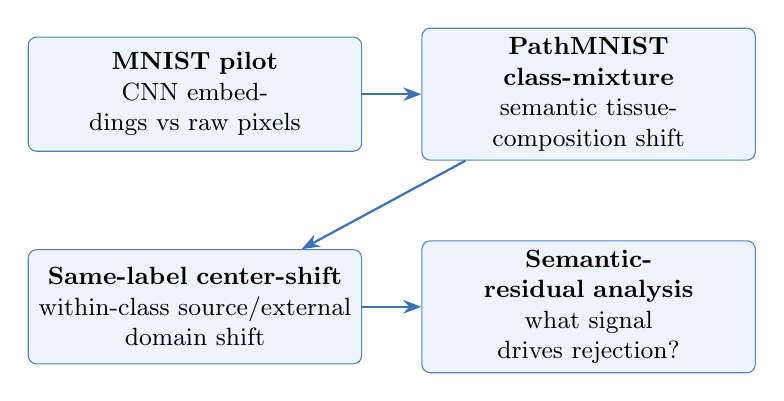
\begin{tikzpicture}[
  box/.style={
    draw=fudanblue!70,
    fill=fudanlight,
    rounded corners=3pt,
    text width=4.0cm,
    minimum height=1.45cm,
    align=center,
    font=\small
  },
  arr/.style={-{Stealth[length=2.3mm]}, thick, draw=fudanblue!80}
]

\node[box] (a) at (0, 3.7) {
  \textbf{MNIST pilot}\\
  CNN embeddings vs raw pixels
};

\node[box] (b) at (5.0, 3.7) {
  \textbf{PathMNIST class-mixture}\\
  semantic tissue-composition shift
};

\node[box] (c) at (0, 1) {
  \textbf{Same-label center-shift}\\
  within-class source/external domain shift
};

\node[box] (d) at (5.0, 1) {
  \textbf{Semantic-residual analysis}\\
  what signal drives rejection?
};

\draw[arr] (a) -- (b);
\draw[arr] (b) -- (c);
\draw[arr] (c) -- (d);

\end{tikzpicture}
\end{center}

\vspace{1.0cm}
\end{frame}

% -------------------------------------------------------------------
\begin{frame}{PathMNIST Class-Mixture}{Semantic tissue-composition shift}
\begin{columns}[T,totalwidth=\linewidth]
\begin{column}{0.57\linewidth}
  \fig[width=1.03\linewidth]{pathmnist_class_mixture_power.png}
\end{column}
\begin{column}{0.38\linewidth}
  {\large\bfseries Task}\\[0.25em]
  \texttt{mix635} vs \texttt{mix835}: two shared tissue components, one component changed.

  \vspace{0.65em}
  {\large\bfseries Result}\\[0.25em]
  CNN final and multilayer embeddings improve power over raw pixels.

  \vspace{0.45em}
  \small
  \begin{center}
  \begin{tabular}{lrr}
  \toprule
  Method & $n=90$ & $n=120$ \\
  \midrule
  Raw pixel & 0.497 & 0.636 \\
  FC-128 & 0.774 & \textbf{0.963} \\
  Multilayer G15 & \textbf{0.796} & 0.959 \\
  \bottomrule
  \end{tabular}
  \end{center}
\end{column}
\end{columns}
\end{frame}

% -------------------------------------------------------------------
\begin{frame}{Class-Mixture Type-I Check}{Matched null: \texttt{mix635} vs \texttt{mix635}}
\keyline{Matched-null rejection stays below $\alpha=0.05$.}
\vspace{-0.16cm}
\begin{center}
  \fig[width=0.78\linewidth]{pathmnist_class_type1_zoom.png}
\end{center}
\end{frame}

% -------------------------------------------------------------------
\begin{frame}{Same-Label Center Shift}{A biomedical domain-shift test}
\begin{center}
  \fig[width=0.90\linewidth]{pathmnist_center_shift_examples.png}
\end{center}
\vspace{-0.20cm}
\begin{center}
\hspace*{0.12cm}\begin{minipage}{0.92\linewidth}
\begin{columns}[T,totalwidth=\linewidth]
\begin{column}{0.46\linewidth}
  \centering\small\textbf{\pos{Source / internal}}: official train holdout.
\end{column}
\begin{column}{0.46\linewidth}
  \centering\small\textbf{\warn{External}}: official external test center.
\end{column}
\end{columns}
\end{minipage}
\end{center}
\end{frame}

% -------------------------------------------------------------------
\begin{frame}{Center-Shift Result}{Same-label shift is strong, but representation profiles differ}

\vspace{-0.15cm}

\begin{center}
  \fig[width=0.78\linewidth]{pathmnist_center_shift_power.png}
\end{center}

\vspace{-0.10cm}

\begin{center}
\begin{minipage}[t]{0.36\linewidth}
\centering
{\normalsize\bfseries Rejection rate at $n=50$}\\[0.15em]
\scriptsize
\begin{tabular}{@{}lrr@{}}
\toprule
Method & Label 6 & Label 8 \\
\midrule
Raw pixel & 0.782 & 0.960 \\
FC-128 & 0.763 & 0.957 \\
Multilayer G15 & 0.989 & 0.975 \\
Multilayer single & \textbf{0.991} & \textbf{0.985} \\
\bottomrule
\end{tabular}
\end{minipage}
\hspace{0.035\linewidth}
\begin{minipage}[t]{0.43\linewidth}
\vspace{0.05cm}
\begin{itemize}
  \item Label 6: multilayer is much stronger than raw / FC-128.
  \item Label 8: raw pixel and FC-128 are already strong.
  \item Representation profile differs by label; next we try to locate the signal.
\end{itemize}
\end{minipage}
\end{center}

\end{frame}

% -------------------------------------------------------------------
\begin{frame}{Semantic vs Residual Signal}{What part of FC-128 drives rejection?}

\vspace{0.02cm}

{\normalsize
In a same-label test, MMMD rejection may come from different directions of the CNN representation.
}

\vspace{-0.12cm}

\begin{center}
\normalsize
\[
\text{logits}=Wh+b,\qquad
W_c=\left(I-\frac{1}{C}\mathbf{1}\mathbf{1}^{T}\right)W,\qquad
h=h_{\mathrm{sem}}+h_{\mathrm{res}}.
\]
\end{center}

\vspace{0.28cm}

\begin{center}
\begin{minipage}{0.94\linewidth}
\begin{columns}[T,totalwidth=\linewidth]

\begin{column}{0.48\linewidth}
\centering
{\large\bfseries Classifier-used part}\\[0.38em]
{\large $h_{\mathrm{sem}}=P_{\mathrm{row}(W_c)}h$}\\[0.22em]
\begin{minipage}{0.88\linewidth}
\begin{itemize}
  \item affects class-relative logits
  \item aligned with tissue-discriminative directions
\end{itemize}
\end{minipage}
\end{column}

\begin{column}{0.48\linewidth}
\centering
{\large\bfseries Classifier-ignored part}\\[0.38em]
{\large $h_{\mathrm{res}}=h-h_{\mathrm{sem}}$}\\[0.22em]
\begin{minipage}{0.88\linewidth}
\begin{itemize}
  \item invisible to the linear classifier head
  \item may still contain domain or stain signal
\end{itemize}
\end{minipage}
\end{column}

\end{columns}
\end{minipage}
\end{center}

\vspace{0.30cm}

\begin{center}
{\scriptsize Diagnostic decomposition: used to interpret the rejection source, not to claim FC-128 is always strongest.}
\end{center}

\end{frame}

% -------------------------------------------------------------------
\begin{frame}{Semantic--Residual Result}{Task $\times$ component readout}
\keyline{Class-mixture is semantic/logit-aligned; label-8 center shift is residual-dominated.}
\vspace{0.10cm}
\begin{center}
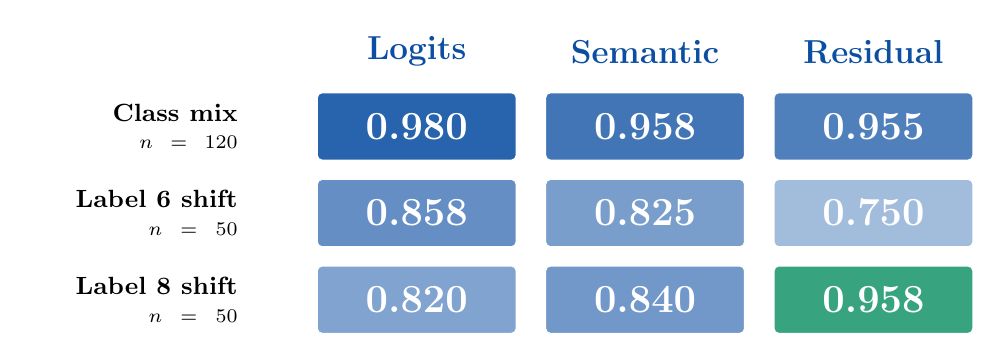
\begin{tikzpicture}[
  cell/.style={draw=white,line width=1.1pt,rounded corners=2pt,
               minimum width=2.55cm,minimum height=0.88cm,
               align=center,font=\Large\bfseries},
  rowlab/.style={anchor=east,text width=2.55cm,align=right,font=\small\bfseries},
  head/.style={font=\large\bfseries\color{fudanblue}}
]
  \node[head] at (2.05,3.05) {Logits};
  \node[head] at (4.95,3.05) {Semantic};
  \node[head] at (7.85,3.05) {Residual};

  \node[rowlab] at (-0.10,2.10) {Class mix\\[-1pt]\scriptsize $n=120$};
  \node[cell,fill=fudanblue!88,text=white] at (2.05,2.10) {0.980};
  \node[cell,fill=fudanblue!78,text=white] at (4.95,2.10) {0.958};
  \node[cell,fill=fudanblue!72,text=white] at (7.85,2.10) {0.955};

  \node[rowlab] at (-0.10,1.00) {Label 6 shift\\[-1pt]\scriptsize $n=50$};
  \node[cell,fill=fudanblue!63,text=white] at (2.05,1.00) {0.858};
  \node[cell,fill=fudanblue!55,text=white] at (4.95,1.00) {0.825};
  \node[cell,fill=fudanblue!38,text=white] at (7.85,1.00) {0.750};

  \node[rowlab] at (-0.10,-0.10) {Label 8 shift\\[-1pt]\scriptsize $n=50$};
  \node[cell,fill=fudanblue!52,text=white] at (2.05,-0.10) {0.820};
  \node[cell,fill=fudanblue!58,text=white] at (4.95,-0.10) {0.840};
  \node[cell,fill=accentgreen!78,text=white] at (7.85,-0.10) {0.958};
\end{tikzpicture}
\end{center}
\vspace{0.18cm}
\begin{center}
\smallnote{Entries are MMMD rejection rates at representative sample sizes.}
\end{center}
\end{frame}

% -------------------------------------------------------------------
\begin{frame}{Label-8 Residual Checks}{Residual signal survives dimension matching and concentrates in few PCs}
\keyline{Label-8 shift is residual-dominated and low-dimensional.}
\vspace{-0.10cm}
\begin{center}
  \fig[width=0.94\linewidth]{label8_residual_checks_two_panel.png}
\end{center}
\end{frame}

% -------------------------------------------------------------------
\begin{frame}{Color/Stain Explanation I}{Color15 explains residual domain score}
\keyline{Color/stain explains a large part of the label-8 residual shift.}
\vspace{-0.12cm}
\begin{center}
  \fig[width=0.88\linewidth]{color_domain_score_explained.png}
\end{center}
\end{frame}

% -------------------------------------------------------------------
\begin{frame}{Color/Stain Explanation II}{Color15 $\to$ propensity matching $\to$ residual MMMD}
\keyline{Color matching weakens residual signal; do not overclaim morphology.}
\vspace{-0.12cm}
\begin{center}
  \fig[width=0.88\linewidth]{color_mmmd_matching_summary.png}
\end{center}
\end{frame}

% -------------------------------------------------------------------
\end{document}
